%\documentclass[12pt]{report} 
\documentclass[12pt,times]{elsarticle}
\topmargin -25mm

\textheight 24truecm   
\textwidth 16truecm    
\oddsidemargin 1mm
\evensidemargin 1mm   
\setlength\parskip{10pt}
\pagestyle{empty}          

%\usepackage{boxedminipage}
\usepackage{amsfonts}
\usepackage{amsmath} 
\usepackage{amssymb}
\usepackage{graphicx}
%\usepackage{bbm,booktabs}
%\usepackage{lipsum}
%\usepackage{multicol}
\usepackage[colorlinks=true, urlcolor=blue]{hyperref}


\makeatletter
\def\ps@pprintTitle{%
\let\@oddhead\@empty
\let\@evenhead\@empty
\def\@oddfoot{}%
\let\@evenfoot\@oddfot}
\makeatother


\begin{document}
	\title{A Network Perspective on LDA}
	\author{Cindy Cook \\ \normalsize Network Analysis Final Project \\ \normalsize April 2015}
	\date{}
	\maketitle

\section{Introduction}
\vspace{-4mm}
With an increase in the amount of digitized text, topic modeling has become an important area of research. One of the most popular methods for topic modeling is Latent Dirichlet Allocation (LDA) first described in \cite{lda}. LDA, a probabilistic hierarchical generative model, uses the Bayesian framework to discover hidden structure, or \textit{topics},  within a set of documents referred to as a corpus. Given a document, the distribution of latent topics is found through estimation of the posterior distribution. Although LDA is commonly used, the methods are called into question by Lancichinetti in \cite{main}. More info here...
\par
This paper begins by describing a data set, referred to as Science using both descriptive and network statistics, that can be found in \cite{main}. It then replicates the main findings from \cite{main} involving the Science dataset. Lastly, we focus on expanding the study by...

\subsection{The Data}
\vspace{-4mm}
All data and scripts can be found on github \href{https://github.com/cmcook22/Cook_Networks_Project}{here} . There are two main `real world' datasets used to test the TopicMapping algorithms:  Science and Wikipedia. The Science corpus contains $28,838$ documents from the web of science, where each document contains the title and abstract of a paper published in one of six top journals from different disciplines. After preprocessing the data, there are $106,143$ unique words and over $8.7 \times 10^{6}$ edges. The Wikipedia dataset contains over $4 \times 10^{6}$ nodes with over $800 \times 10^{6}$ edges. Due to the size of the Wikipedia data set, I was unable to receive this information from the authors. Therefore, I will focus on the Science data set only. Although the Science corpus was easily sent to me, it is still considered `large.' In R, the adjacency matrix is too large to be stored. In particular, the program crashes while trying to plot the network using the plot function in the network package. In order to visually see the network, I used only the first $10$ documents to create a network.

\begin{figure}[h!]
	\centering
	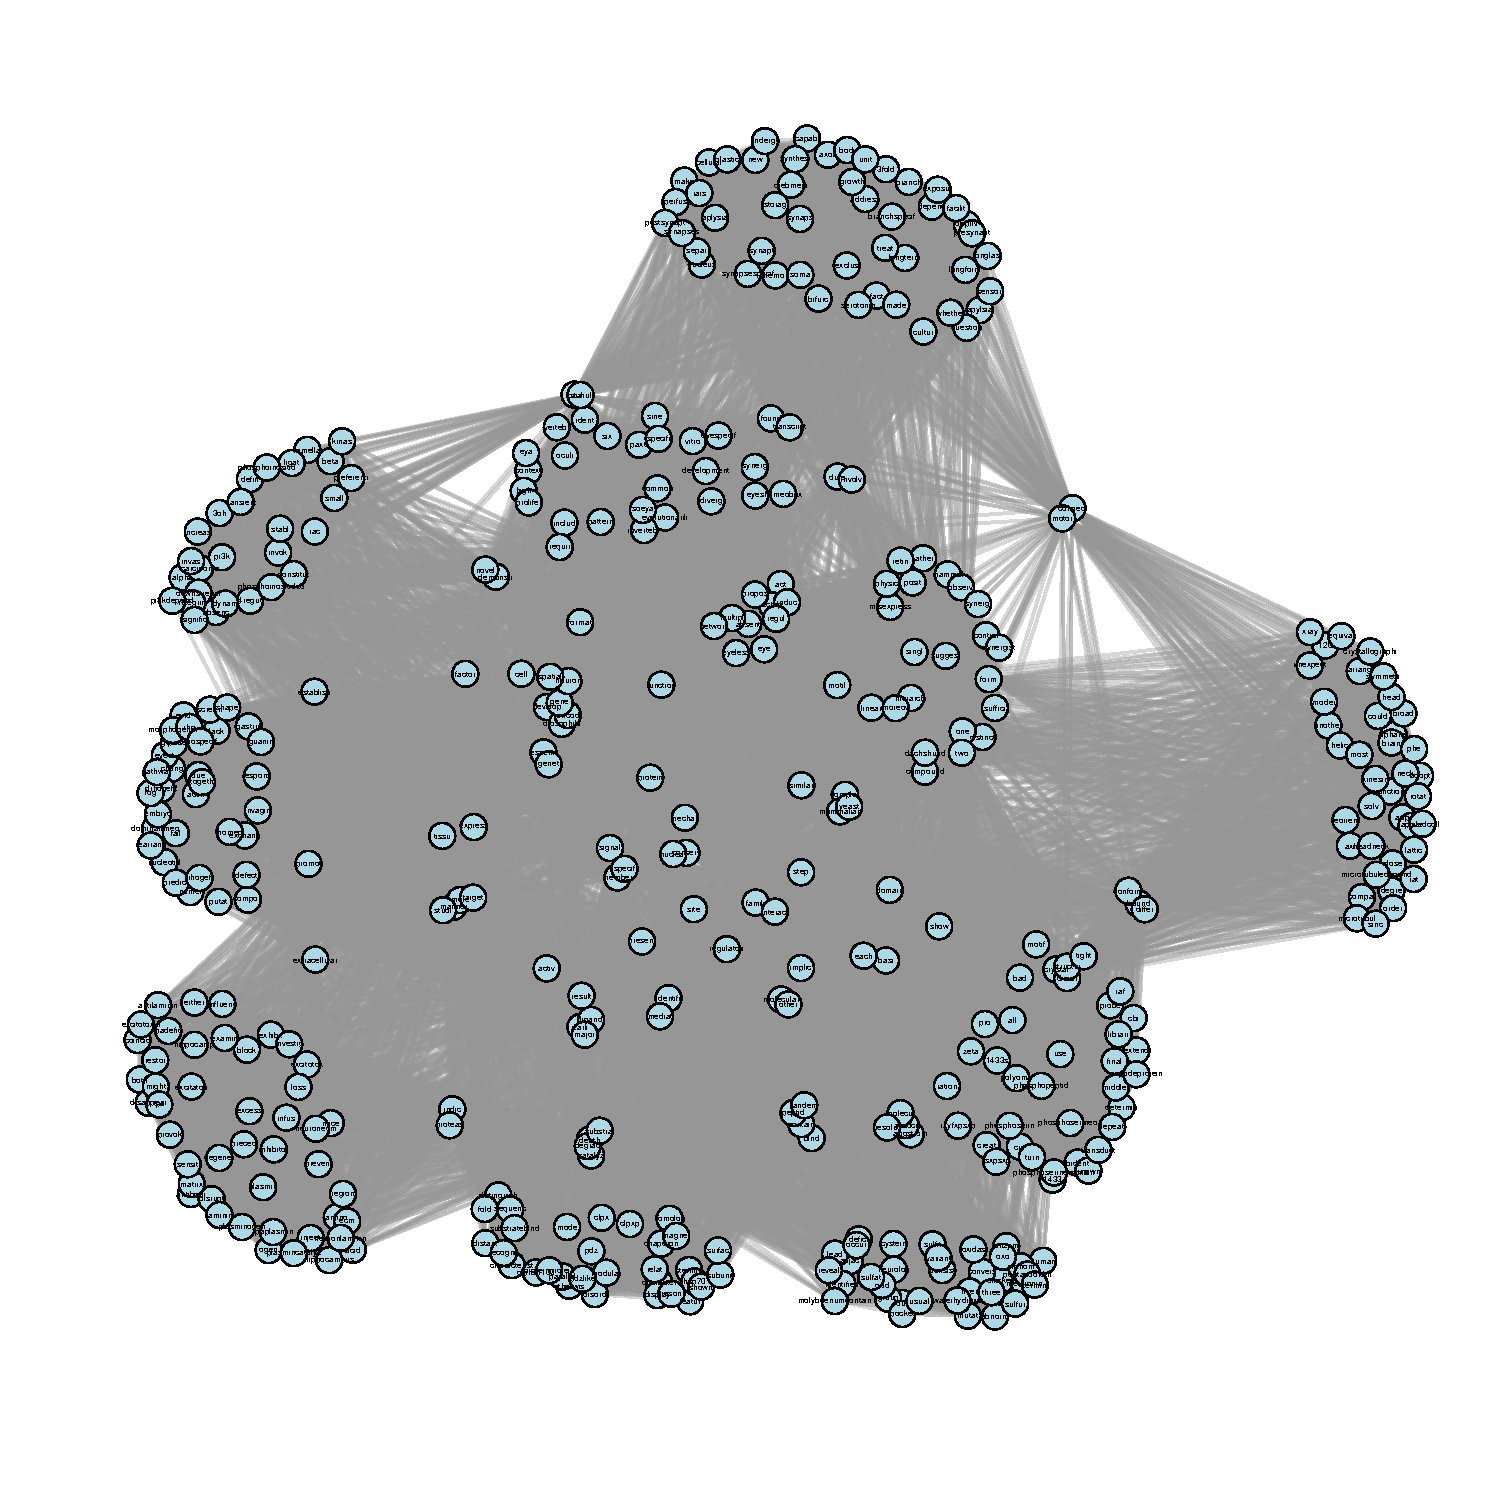
\includegraphics[width=70mm,height=60mm]{Images/simple_plot.pdf}
	\caption{Network Plot of the first $10$ Documents \label{fig.1}}
\end{figure} 

What we immediatley see in this plot are very distinct clusters along with very distinct bridges. Explain what this is informing us here...
The article also makes use of several synthetic datasets: list and explain here for what I will use...

\section{Replicate the Study}
\vspace{-4mm}


\section{Further the Study}
\vspace{-4mm}


\section{Conclusions}
\vspace{-4mm}
\subsection{Discussion}
\vspace{-2mm}

\subsection{Future Directions}
\vspace{-2mm}





\newpage
\section{Bibliography}
\begin{thebibliography}{4}
		
	\bibitem{lda}
	Blei, D., Ng, A., and Jordan, M.  (2003),
	``Latent Dirichlet Allocation."
	\textit{Journal of Machine Learning Research}: 3 993-1022.
	
	\bibitem{main}
	Lancichinetti, A., Sirer, M., Wang, J., Acuna, D., Kording, K., and Amaral, Luis. (2015),
	``High-Reproducibility and High-Accuracy Method for Automated Topic Classification."
	\textit{Physical Review X}: 5, 0011007, 2160-3308.
	
\end{thebibliography}





\end{document}